% % % % % % % % % % % % % % % % % % % % % % % 
% DOCUMENT SETUP
% % % % % % % % % % % % % % % % % % % % % % % 
\documentclass[12pt]{article}
\usepackage[letterpaper,left=0.75in,right=0.75in,top=1.0in,bottom=1.0in]{geometry}


% % % % % % % % % % % % % % % % % % % % % % % 
% IMPORTED PACKAGES
% % % % % % % % % % % % % % % % % % % % % % % 
\usepackage[utf8]{inputenc}
\usepackage{enumitem}
\usepackage{dsfont}
\usepackage{ulem}
\usepackage{hyperref}
\hypersetup{
    colorlinks=true,
    linkcolor=white,
    urlcolor=blue, 
    breaklinks=true
}
\usepackage{breakcites}
%\usepackage{caption}
\usepackage[version=4]{mhchem}
\usepackage{float}
\usepackage[hang]{subfigure}
\usepackage{overpic}
\usepackage{listings}
\usepackage[super]{nth}
\usepackage{multicol}
\linespread{1.15}
\usepackage{siunitx}
\usepackage{makecell}
\usepackage{booktabs}

% % % % % % % % % % % % % % % % % % % % % % % 
% PROJECT SPECIFICATIONS
% % % % % % % % % % % % % % % % % % % % % % %  
\title{Nickel(II) and Copper(II) Supported Metal Complex Stability in NU-1000 Under Hydrogenation Conditions}
\author{Stephen Vicchio}

% % % % % % % % % % % % % % % % % % % % % % % 
% THE DOCUMENT
% % % % % % % % % % % % % % % % % % % % % % %
\begin{document}
\maketitle

\section{Introduction and Methodology}
\begin{itemize}
    \item  Experimentally, the active site composition of \ce{Cu} metal complexes supported in NU-1000 is a function of reaction conditions. The primary outcomes in this paper are related to  probing the catalyst stability in environments containing \ce{H2} for both \ce{Ni} and \ce{Cu} supported metal complexes as a function of temperature, and \ce{H2} and \ce{H2O} partial pressures. In our analysis, address the following topics:
    \begin{itemize}
        \item Identifying reaction conditions that demonstrate structures with the \ce{M(0)} species in both Cu-NU-1000 and Ni-NU-1000 models. 
        \item Determining if \ce{Cu} NPs form by completely stripping all \ce{Cu} atoms in the cluster or if \ce{Cu} atoms attached to the node remain with the NPs forming from the bridge \ce{Cu} atoms. Elucidating if \ce{Ni} follows the same trends at \ce{Cu} in an \ce{H2} reducing environment. 
        \item 
        If metal atoms remain fixed to the node, what is the composition of those active sites? Are these sites metal hydrides? 
    \end{itemize}
    \item Based on the literature, we selected a molecular model for \ce{Cu} (\ce{Cu3(OH)4})(Ikuno et al., 2017) and \ce{Ni} (\ce{Ni4(OH)6}) (Platero-Prats et al., 2017) that contained supported metal complexes with metal sites spanning the c-pore in NU-1000 (as shown in Figure 1d and 1e).
    \begin{figure}[H]
        \centering
        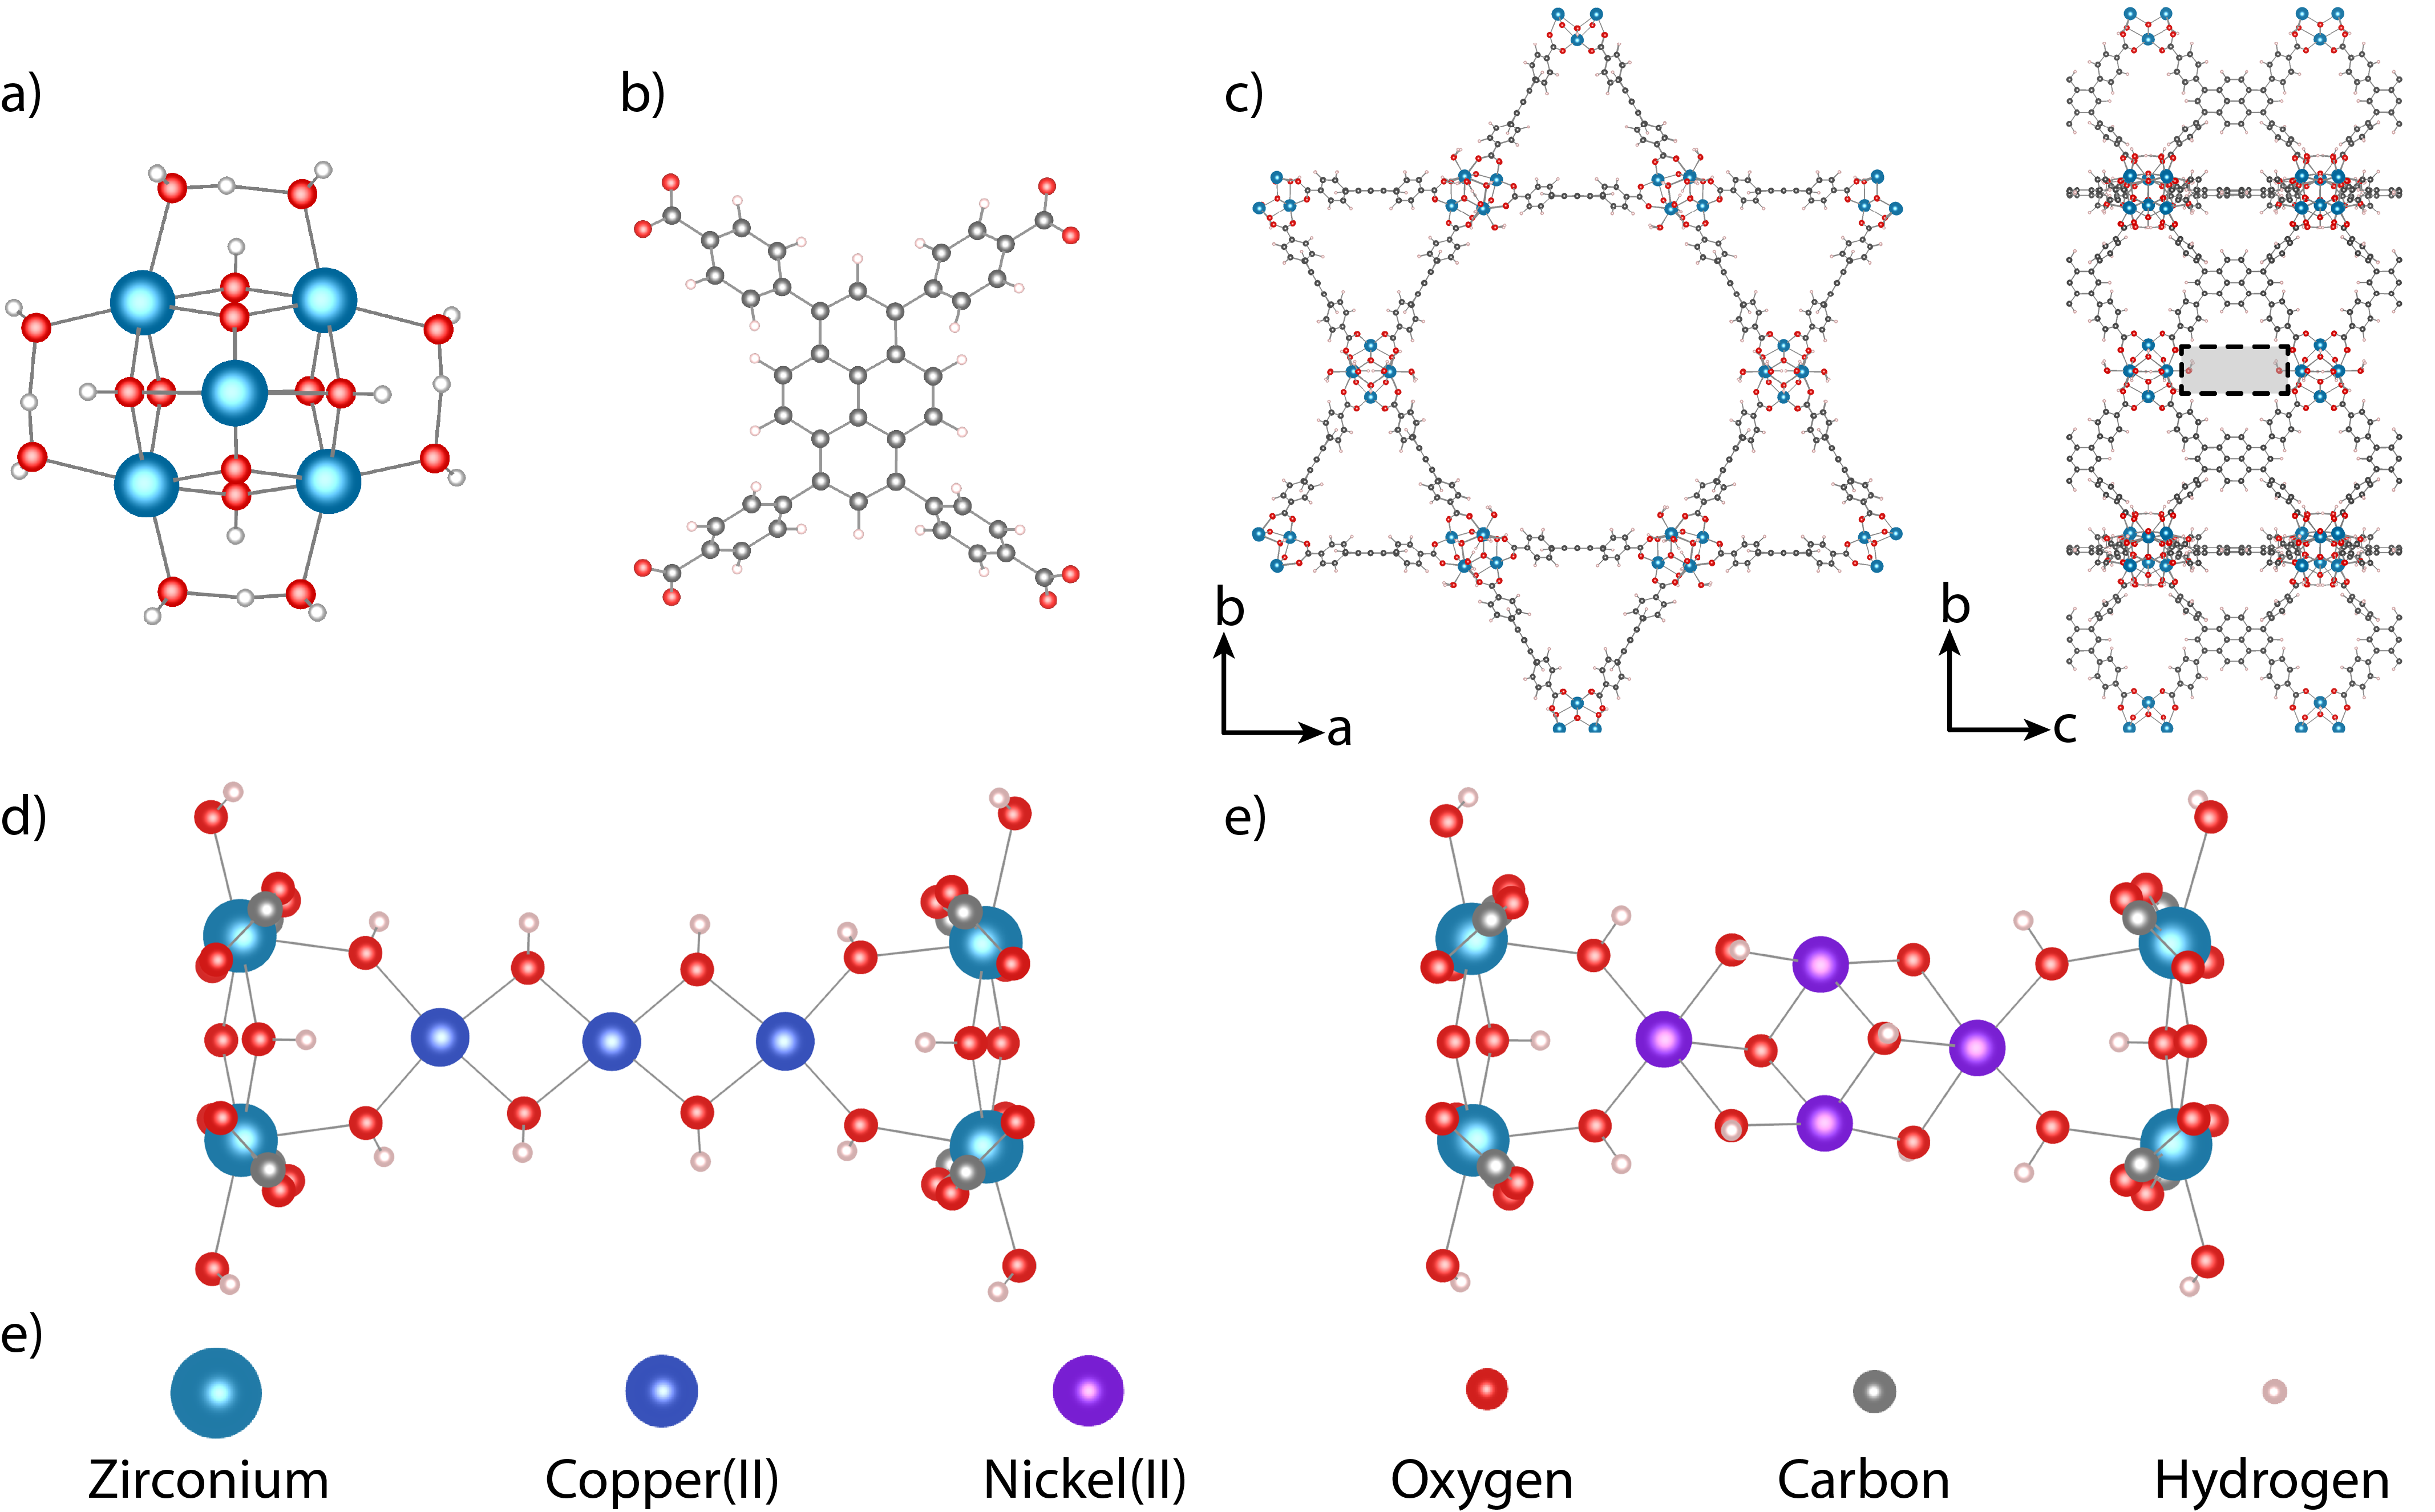
\includegraphics[width=0.95\textwidth]{zi-images/00-General-Graphics/2020-07-31-Combined-MOF-Figure-final.png}
        \caption{The structure of NU-1000, which is comprised of (a)  inorganic nodes (\ce{[Zr6(\mu3-O)4(\mu3-OH)4(H2O)4(OH)4]^8^+}) and (b) organic linkers (1,3,6,8-tetrakis(p-benzoic acid)pyrene (\ce{TBAPy^4^-})) to produce (c) the framework structure (with the c-pore highlighted by the gray box). Additionally, the two metal complexes supported in the c-pore of NU-1000 are also shown: (d) the \ce{Cu3(OH)4} metal complex, and (d) the \ce{Ni4(OH)6} metal complex.}
        \label{fig:MOFstructure}
    \end{figure}
    \item To determine the relative stability of different activated Cu-NU-1000 and Ni-NU-1000 structures, the starting composition is modulated using the following equation (shown below for \ce{Cu}):
    \begin{equation} \label{exp:gibbsfreeoverall}
        \ce{z * H2 + Cu3(OH)4-MOF <=>[$\Delta G(T,P)$] Cu3O_{4-n}H_{4+2z-2n}-MOF + n * H2O}
    \end{equation}
     The structure of the activated cluster is a function of the gas phase conditions. Determining the Gibbs free energy ($\Delta G(T,P)$) for each activated cluster at different reaction conditions provides information on the thermodynamic landscape. The gas phase \ce{H2} and \ce{H2O} chemical potential terms relate the reaction conditions ($T$ and $P$) to $\Delta G(T,P)$. The chemical potential terms are a function of the conditions. 
     \item At specific $T$ and $P$ conditions, the structure with the lowest $\Delta G(T,P)$ was identified. The phase diagrams (shown below) are generated by plotting the low energy structure at all reaction conditions. Approximately 70 structures for \ce{Cu} and 300 structures for \ce{Ni} were modeled to determine the thermodynamic stability. The structures had varying compositions and morphologies including structures with \ce{M-H}, physisorbed \ce{H2O}, and metallic bonds. 
\end{itemize}

\section{Results}
\subsection{Cu-NU-1000}
\begin{itemize}
    \item The \ce{Cu} phase diagram in Figure 2 shows the structural landscape of \ce{Cu3(OH)4} supported in NU-1000, with each region representing a different thermodynamically favorable structure. The phase diagram shows the clusters structurally stability as a function of both \ce{H2} and \ce{H2O} chemical potential terms, which are related to the reaction conditions ($T$ and $P$). Figure 3 shows the structure of each region on the phase diagram and Table 3 provides additional structural information (such as \ce{Cu-Cu} bond distances and \ce{Cu} oxidation state).  
    \begin{figure}[H]
        \centering
        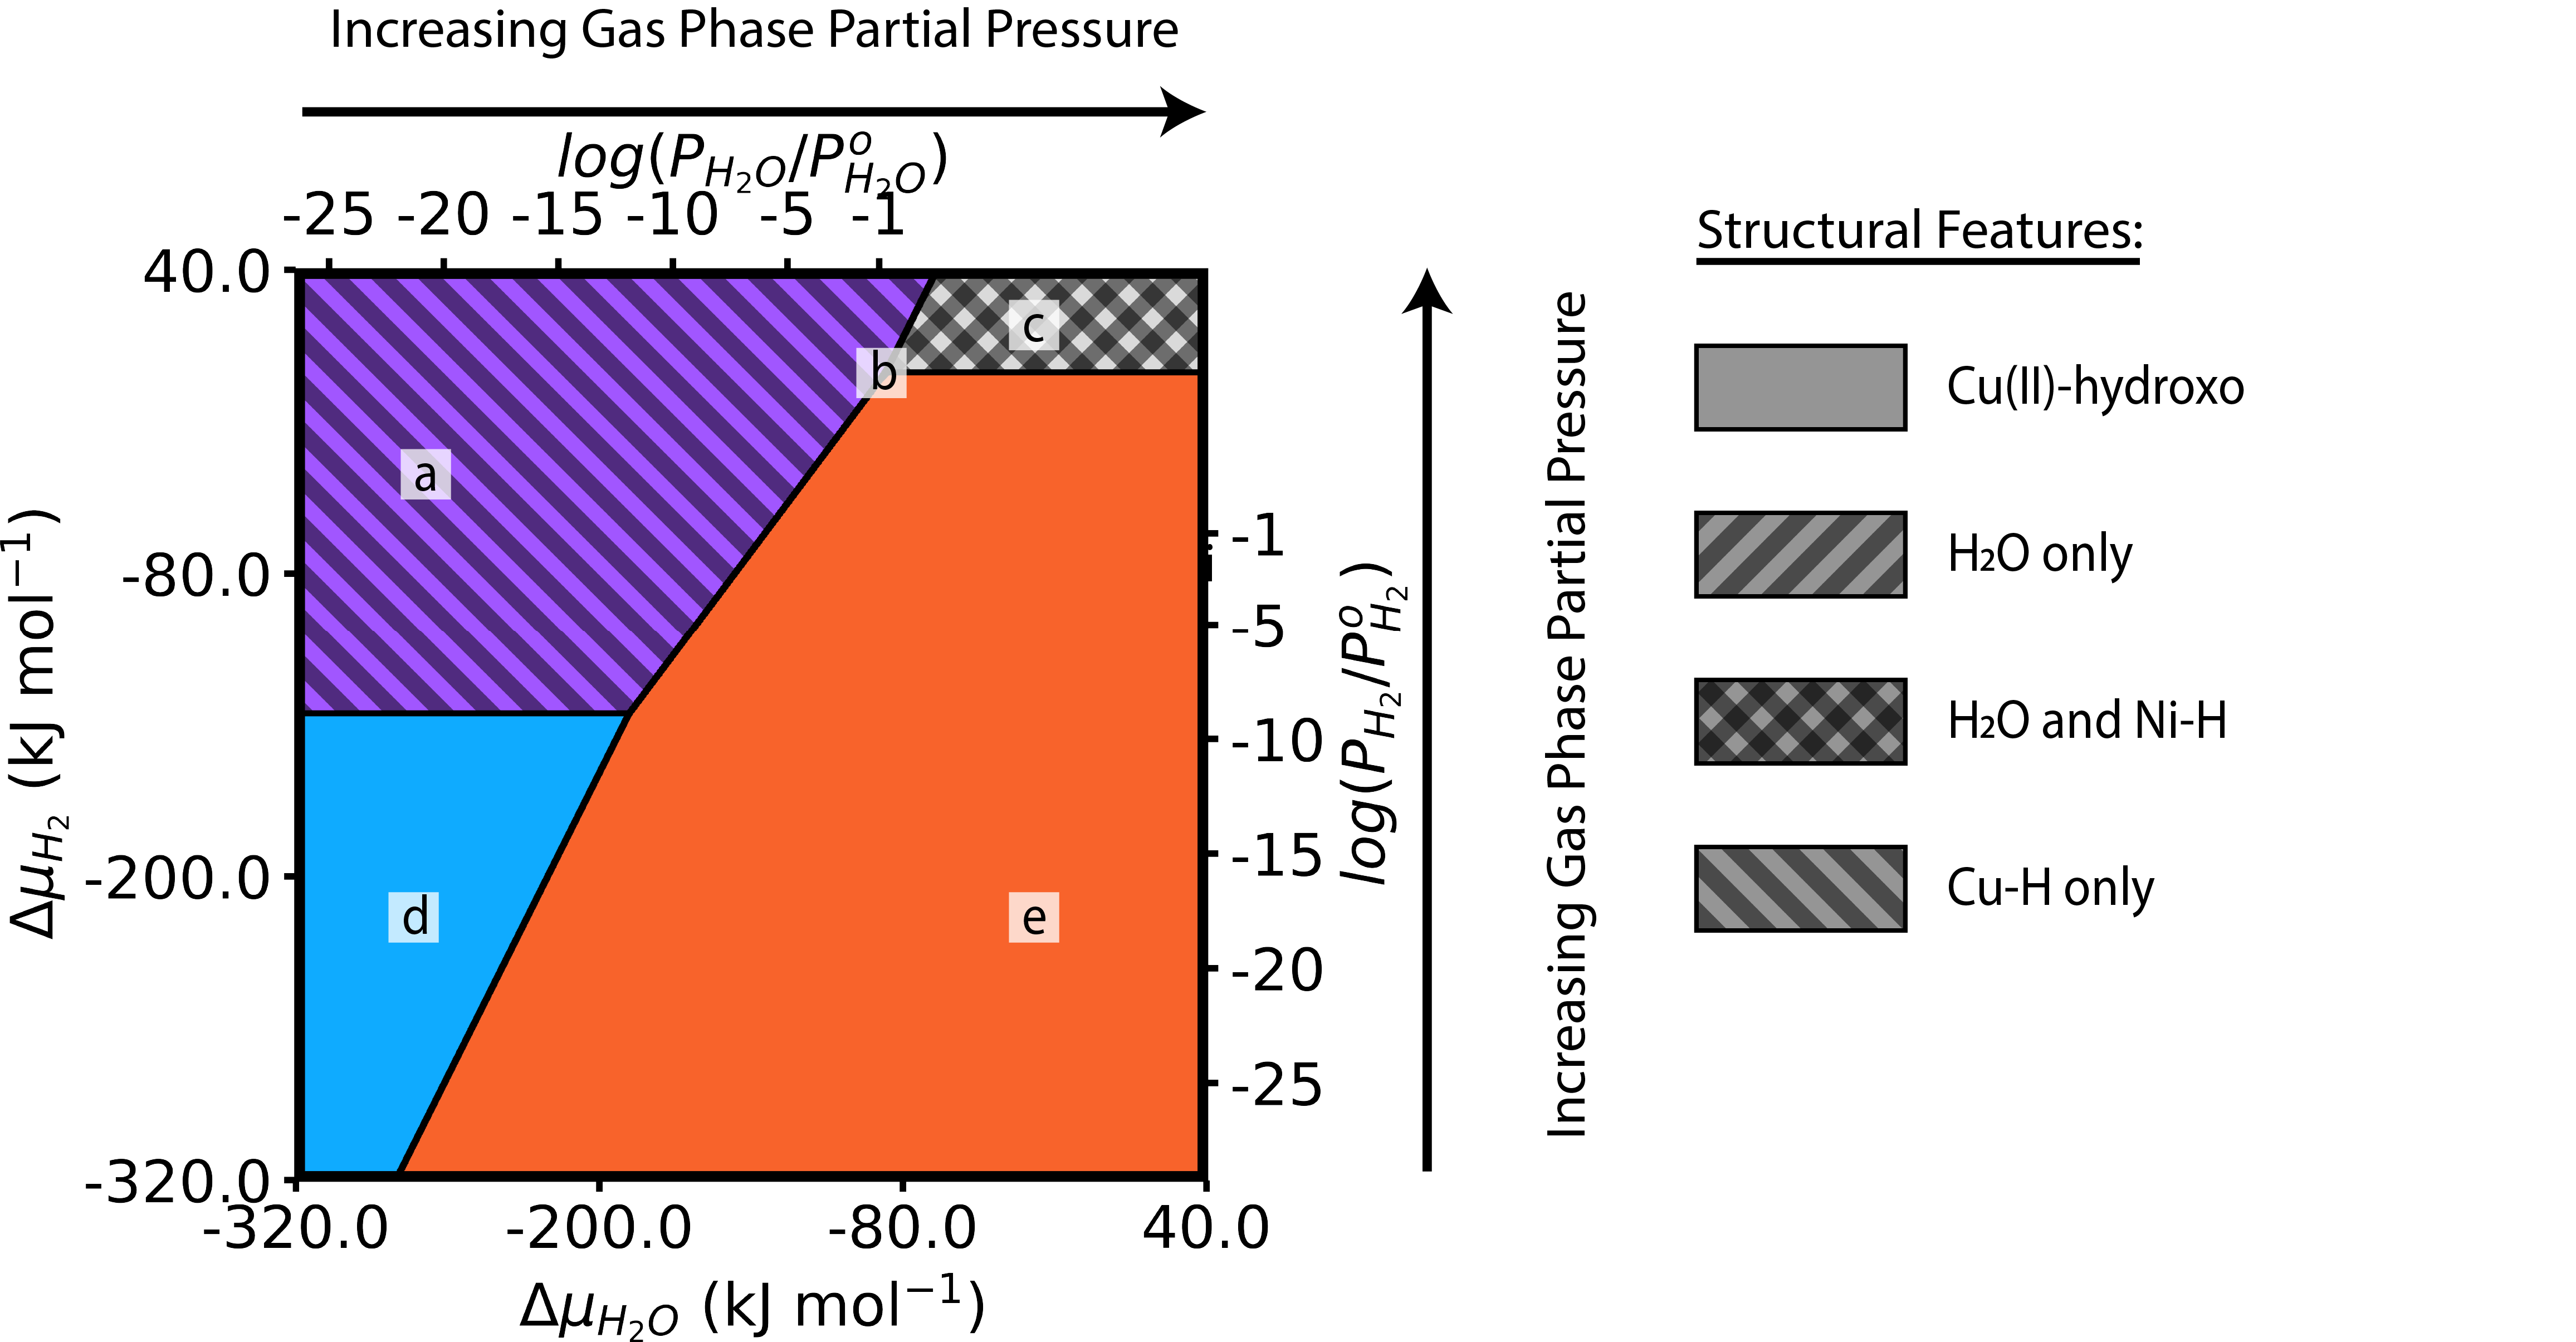
\includegraphics[width=0.95\textwidth]{zi-images/02-Cu-Graphics/2020-08-05-Cu3-phase-diagram-V01.png}
        \caption{Phase diagram generate by \textit{ab initio} thermodynamic analysis that captures the structural stability of a Cu(II) supported metal complex in NU-1000 at \SI{200}{\celsius}. The starting structure is the \ce{Cu3(OH)4} complex. The composition and morphology of the Cu(II) complex changes depending on the \ce{H2} and \ce{H2O} partial pressures, which produces new structural features, such as physisorbed \ce{H2O} and metal hydride structures.}
        \label{fig:phasediagramCu3}
    \end{figure}
    \item Figure 2 reveals five dominate structures containing structural features such as metal hydrides (\ce{Cu-H}) and physisorbed \ce{H2O}. Figure 2e (orange) represents the starting \ce{Cu3(OH)4} structure. The cluster structure is a function of the reaction conditions, revealing different thermodynamic-favorable structural characteristics such as \ce{Cu-H} (Figure 2a, 2b, and 2c), physisorbed \ce{H2O} (Figure 2c), and metallic \ce{Cu-Cu} bonds (figure 2d). 
    \item The physisorbed \ce{H2O} species form by converting one of the \ce{OH}-ligands in the cluster (Figure 2c). The additional proton is from the adsorption of the gas phase \ce{H2}. For \ce{Cu(OH)4}, the structure contains 4 \ce{OH}-ligands that link the \ce{Cu} atoms across the c-pore. Further decreasing the partial pressure of \ce{H2O} allows for the the removal of all \ce{OH}-ligands (Figure 2a and 2d). The structure diagram provides structural information for these changes. 
    \item The weakly bound \ce{H2O} (Figure 2c) desorbs from the cluster (Figure 2b) as the gas phase \ce{H2O} partial pressure decreases. 
    \item The \ce{Cu-H} metal hydride species become favorable under high partial pressure of \ce{H2}. For the \ce{Cu} model, the metal hydrides that form 'bridge' two \ce{Cu} atoms. Figure 3a, 3b, and 3c show the bridging \ce{Cu-H-Cu} structures. The metal hydrides occupy the site of \ce{OH}-ligands. 
    \begin{table}[h]
        \setlength\tabcolsep{8pt}
        \centering
        \caption{Copper Oxidation and \ce{Cu-Cu} Distances}
        \label{tbl:Cu3oxidationstates}
        \begin{tabular}{lccc}
        \hline
            Structure  &  \thead{\ce{Cu} Formal \\ Charge\textsuperscript{\emph{a}}} &   \thead{Potential \ce{Cu} \\ Oxidation State} & \thead{\ce{Cu-Cu} \\ Distance (A)} \\
            \hline
            a) \ce{(CuHCuHCu)}                 & $\frac{4}{3}$ & \ce{Cu(0)}, \ce{Cu(II)}, \ce{Cu(II)}       & 2.96, 3.10  \\
            b) \ce{(CuHCu)(Cu)(OH)3}           & 2             & \ce{Cu(II)}, \ce{Cu(II)}, \ce{Cu(II)}      & 2.81, 3.02  \\
            c) \ce{(CuHCu)Cu(OH)3 \cdot 1H2O}  & 2             & \ce{Cu(II)}, \ce{Cu(II)}, \ce{Cu(II)}      & 2.83, 3.03  \\
            d) \ce{(CuCu)(Cu)}                 & $\frac{2}{3}$ & \ce{Cu(0)}, \ce{Cu(I)}, \ce{Cu(I)}         & 2.37  \\
            e) \ce{Cu3(OH)4}                   & 2             & \ce{Cu(II)}, \ce{Cu(II)}, \ce{Cu(II)}      & 2.98, 3.02  \\
            \hline
        \end{tabular} \\
        \textsuperscript{\emph{a}} Formal Charge given on a per Cu atom basis. \\
    \end{table} 
    \item Table 1 shows the average \ce{Cu} formal charges determined for each structure found in Figure 2. The \ce{Cu} formal charge decreases from 2 in \ce{Cu3(OH)4} (structure e) to $\frac{4}{3}$ in \ce{CuHCuHCu} (structure a) to $\frac{2}{3}$ in \ce{(CuCu)(Cu)} (structure d) as the cluster is reduced. The \ce{Cu} formal charge decreasing coincides with the removal of \ce{OH}-ligands from the cluster.
    \item \ce{(CuCu)(Cu)} (structure d) contains a metallic \ce{Cu-Cu} bond based on \ce{Cu-Cu} distance and potential \ce{Cu} oxidation states for the average \ce{Cu} formal charge. We suggest that the \ce{(CuCu)(Cu)} structure (structure d) contains the mobile \ce{Cu(0)} species. 
\end{itemize}

\begin{figure}[H]
    \centering
    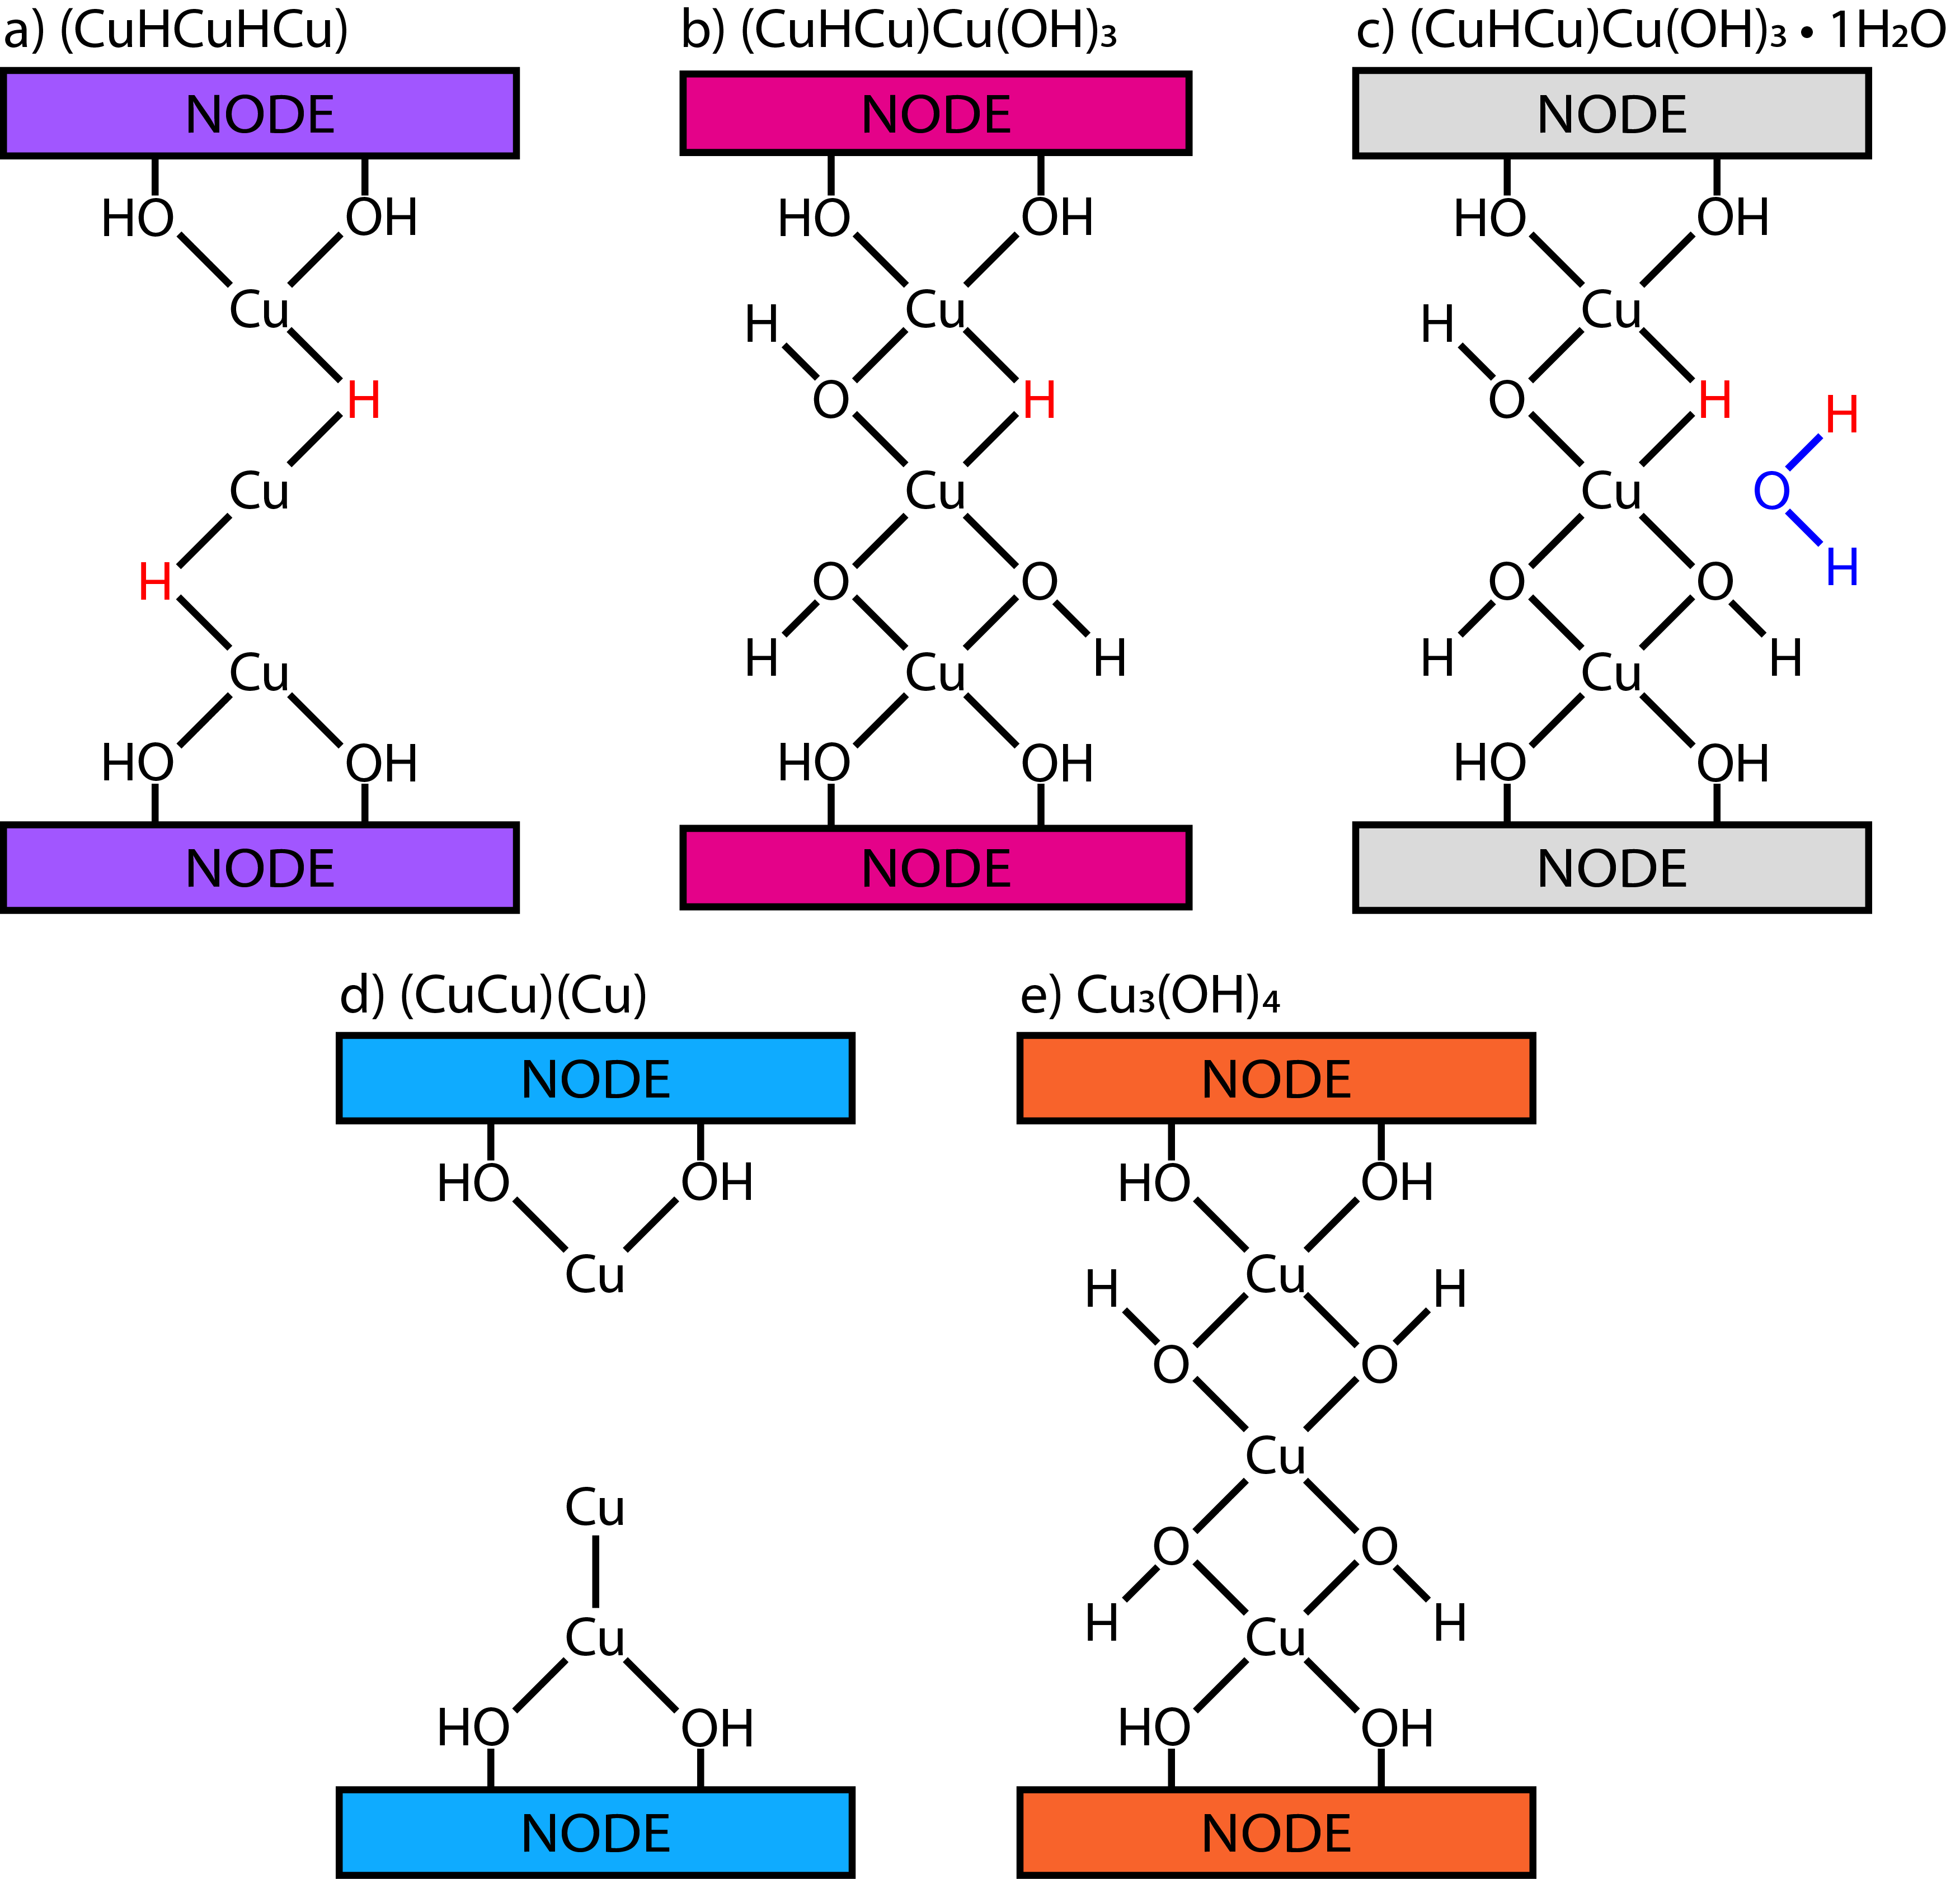
\includegraphics[width=0.70\textwidth]{zi-images/02-Cu-Graphics/2020-08-04-structure-diagram-Cu3OH4-V01-IMAGE.png}
    \caption{Schematic representation of the lowest energy structures from the \textit{ab initio} thermodynamic analysis. The node colors scheme correspond to the \ce{Cu(II)} supported metal complex phase diagram.}
    \label{fig:structurediagramCu3}
\end{figure}

\newpage

\subsection{Ni-NU-1000}
\begin{itemize}
    \item The \ce{Ni4(OH)6} phase diagram (Figure 4) is structurally more diverse than the \ce{Cu3(OH)4} phase diagram (attributed to more metal and \ce{OH}-ligands in the \ce{Ni} metal complex). However, the \ce{Ni4(OH)6} structural features are similar to the features of the \ce{Cu3(OH)4} phase diagram (Figure 2). Both demonstrate metal hydrides, physisorbed \ce{H2O}, and metallic bonds. The structures for phase diagram (Figure 4) are located in Figure 5 and Table 2 contains additional structural information such as \ce{Ni-Ni} bond distances and \ce{Ni} oxidation states. 
    \begin{figure}[H]
        \centering
        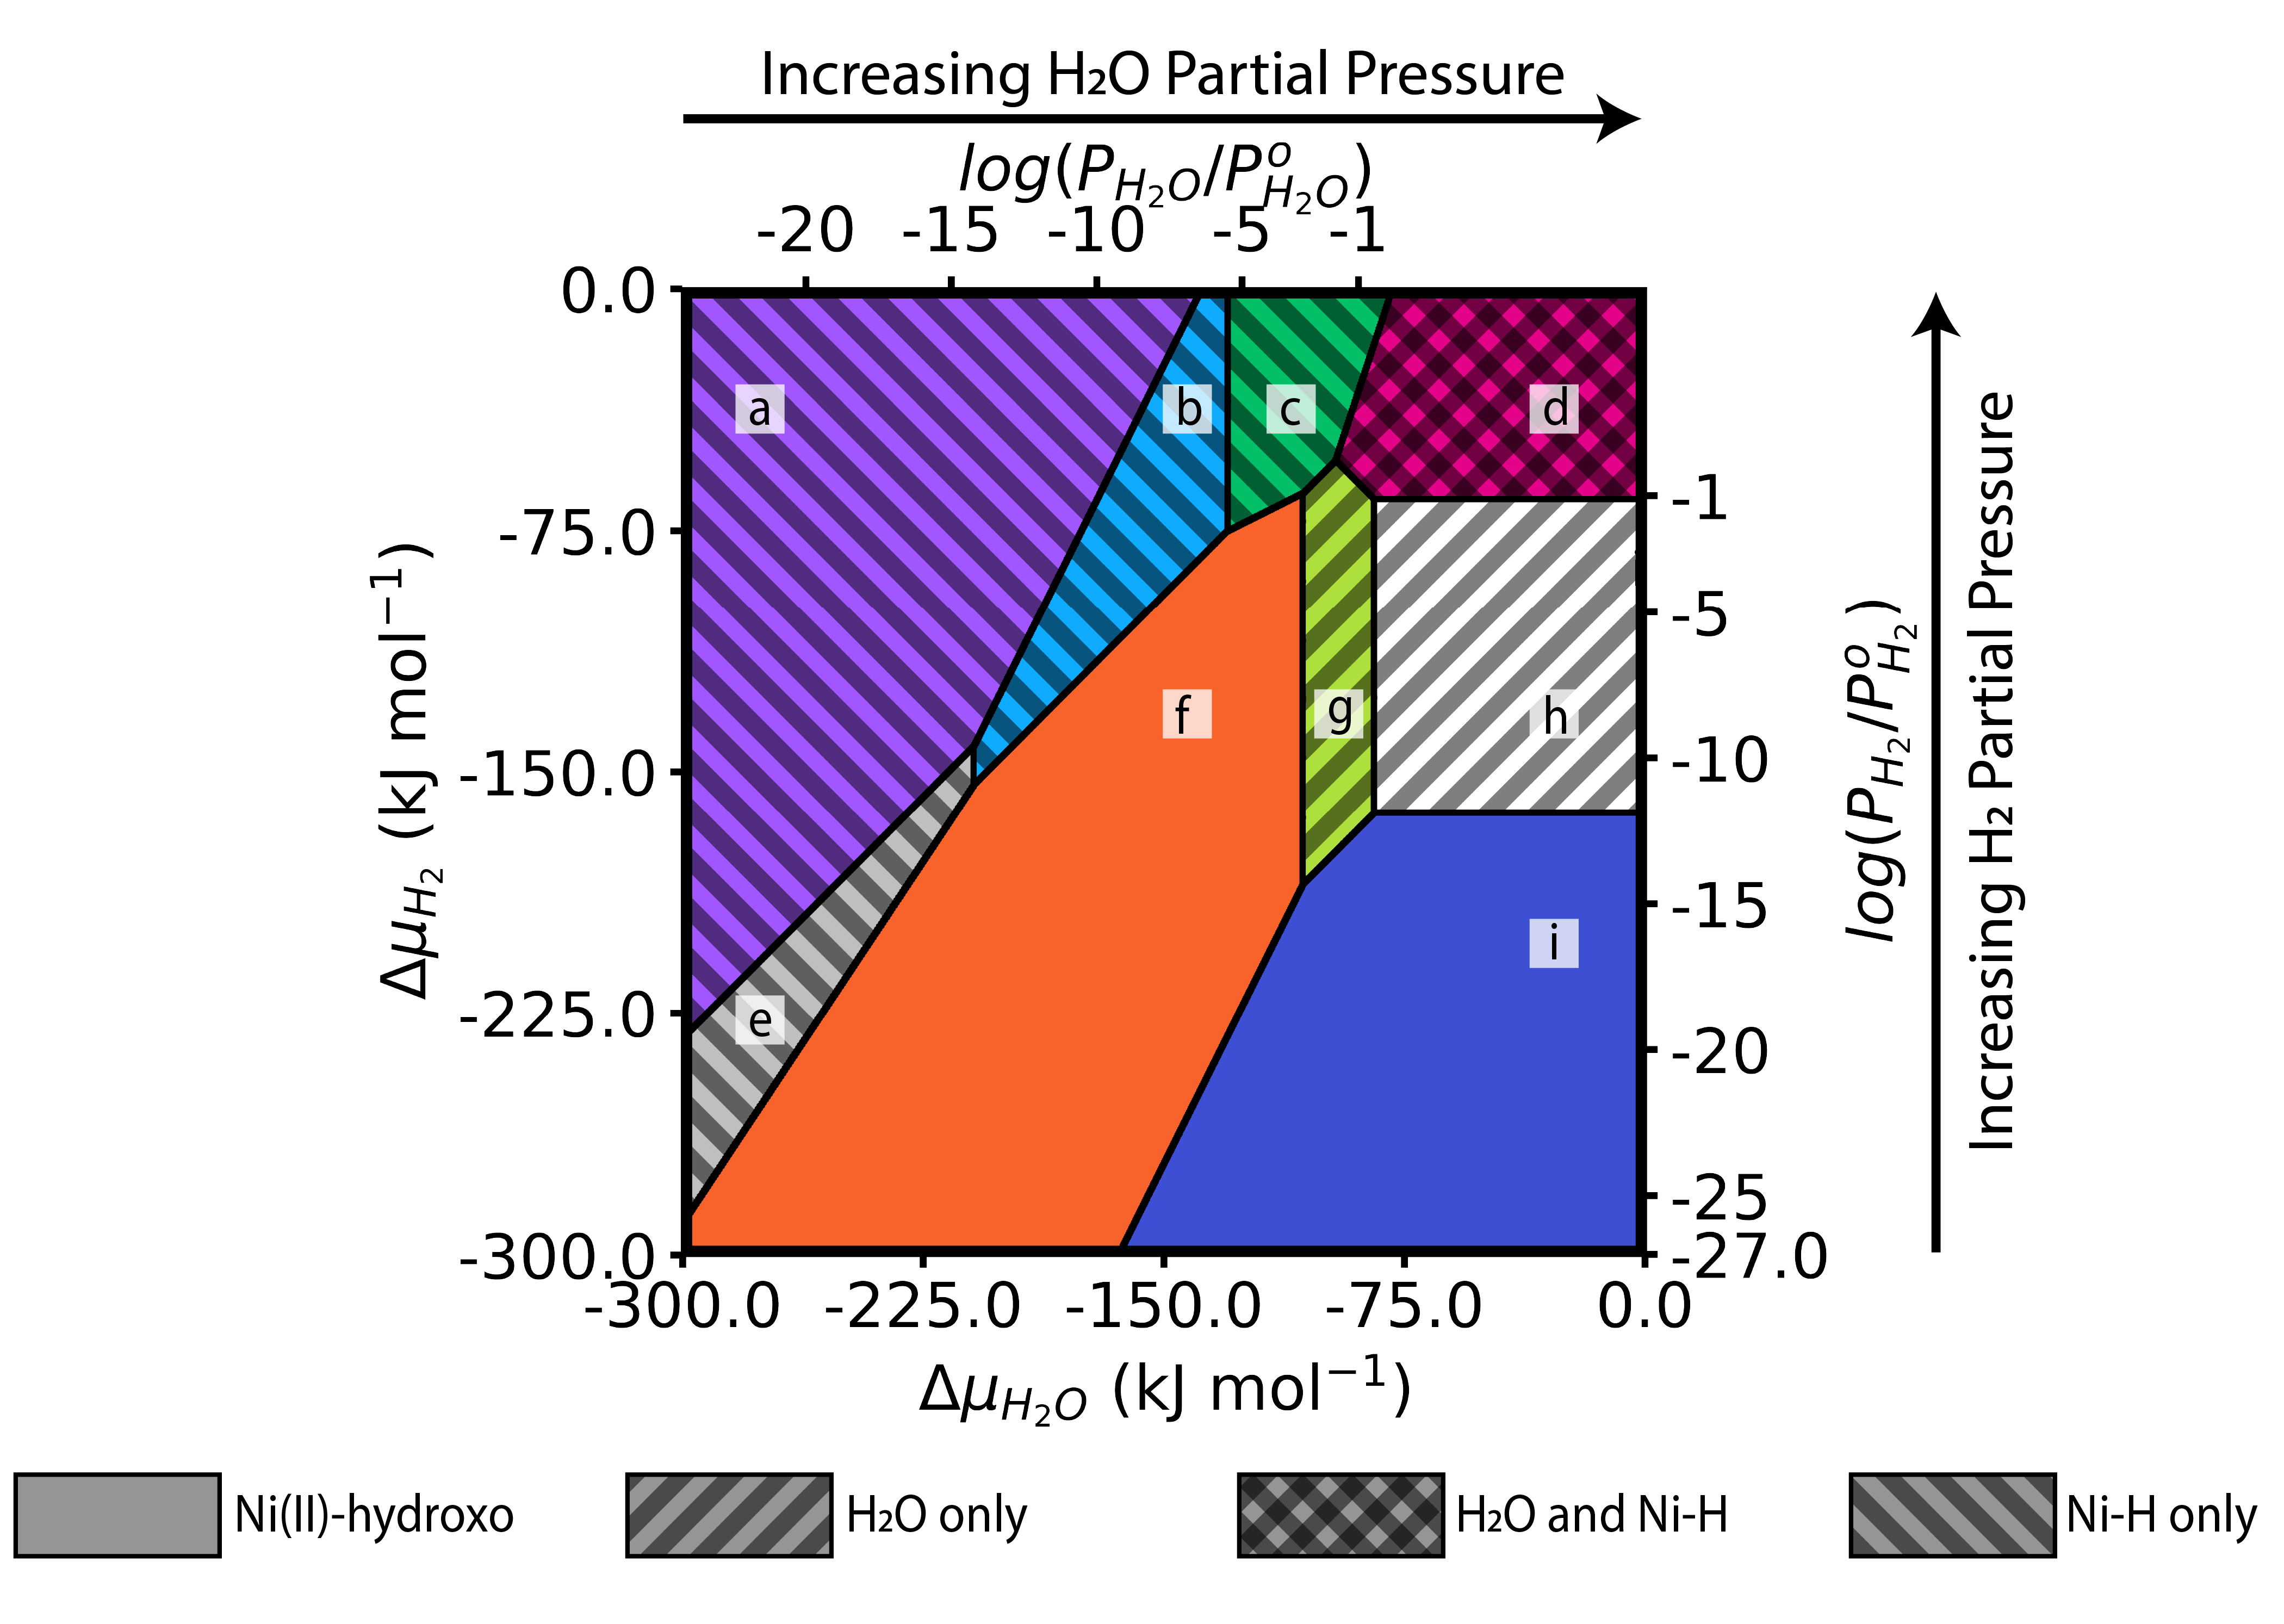
\includegraphics[width=0.85\textwidth]{zi-images/01-Ni-Graphics/2020-08-31-Phase-Diagram-V02.png}
        \caption{Phase diagram generate by \textit{ab initio} thermodynamic analysis that captures the structural stability of a Ni(II) supported metal complex in NU-1000 at \SI{200}{\celsius}. The starting structure is the \ce{Ni4(OH)6} complex. The composition and morphology of the Ni(II) complex changes depending on the \ce{H2} and \ce{H2O} partial pressures, which produces new structural features, such as physisorbed \ce{H2O} and metal hydride structures.}
        \label{fig:phasediagramNi4}
    \end{figure}
    \item If the cluster is exposed to a sufficient \ce{H2} gas the cluster is reduced (the same result as for \ce{Cu}). Table 2 shows a decrease in the \ce{Ni} formal charge. 
    \item The presence of \ce{H2O} in the gas phase has a strong influence over the structurally stability. For example, at \ce{H2} partial pressure of ~ $10^{-1}$ bar, the reduction of the cluster is illustrated going from \ce{Ni2(NiH)2(OH)4 * 2H2O} (structure d) to \ce{(NiH2Ni)(NiNi)} (structure a). 
    \item At higher \ce{H2O} partial pressure, the cluster is more likely to exist as a combination of \ce{Ni-H} and physisorbed \ce{H2O} (structure d and c). As the partial pressure of \ce{H2O} decreases, the formed physisorbed \ce{H2O}s are removed. The \ce{OH}-ligand vacancies are replaced by \ce{H} or left unoccupied. 
    \item The main structures to focus on are the structures that demonstrate the \ce{Ni} reduction from \ce{Ni(II)} to \ce{Ni(0)}. These structures reveal the presence of metallic \ce{Ni} bonds. This zero-valent \ce{Ni} atoms are determined based on \ce{Ni-Ni} distance and the \ce{Ni} formal charge (as shown in Table 2). \ce{Ni-Ni} bond distances between 2.2 A and 2.3, as seen by Structures a, b, c, and e. 
    \begin{table}[h]
        \centering
        \setlength\tabcolsep{8pt}
         \caption{Nickel Formal Charge and \ce{Ni-Ni} Bond Distances.}
         \label{tbl:Ni4oxidationstates}
         \begin{tabular}{lccc}
           \hline
               Structure  &  \thead{\ce{Ni} Formal \\ Charge\textsuperscript{\emph{a}}} &    \thead{Potential \ce{Ni} \\ Oxidation State} & \thead{\ce{Ni-Ni} \\ Distance (A)} \\
           \hline 
           a) \ce{(NiH2Ni)(NiNi)}             & 1             & \ce{Ni(0)}, \ce{Ni(I)}, \ce{Ni(I)}, \ce{Ni(II)}     & 2.23, 2.42 \\   
           b) \ce{(Ni3H2)(Ni)(OH)2}           & $\frac{3}{2}$ & \ce{Ni(I)}, \ce{Ni(I)}, \ce{Ni(II)}, \ce{Ni(II)}     & 2.21, 2.54 \\ 
           c) \ce{(NiH)(Ni3H)(OH)2 * 1H2O}    & $\frac{3}{2}$ & \ce{Ni(0)}, \ce{Ni(II)}, \ce{Ni(II)}, \ce{Ni(II)}     & 2.27, 2.31 \\   
           d) \ce{(Ni2)(NiH)2(OH)4 * 2H2O}    & 2             & \ce{Ni(II)}, \ce{Ni(II)}, \ce{Ni(II)}, \ce{Ni(II)}     & 2.72, 3.17 \\     
           e) \ce{(Ni2H)(NiNi)(OH)}           & 1             & \ce{Ni(0)}, \ce{Ni(I)}, \ce{Ni(I)}, \ce{Ni(II)}     & 2.24, 2.50 \\  
           f) \ce{Ni4(OH)4}                   & $\frac{3}{2}$ & \ce{Ni(I)}, \ce{Ni(I)}, \ce{Ni(II)}, \ce{Ni(II)}   & 2.27, 3.06 \\
           g) \ce{Ni4(OH)4 \cdot 1H2O}        & $\frac{3}{2}$ & \ce{Ni(I)}, \ce{Ni(I)}, \ce{Ni(II)}, \ce{Ni(II)}   & 2.29, 2.96 \\
           h) \ce{Ni4(OH)4 \cdot 2H2O}        & $\frac{3}{2}$ & \ce{Ni(I)}, \ce{Ni(I)}, \ce{Ni(II)}, \ce{Ni(II)}   & 2.33, 3.03 \\
           i) \ce{Ni4(OH)6}                   & 2             & \ce{Ni(II)}, \ce{Ni(II)}, \ce{Ni(II)}, \ce{Ni(II)} & 2.81, 3.03 \\
           \hline
         \end{tabular} \\
         \textsuperscript{\emph{a}} Formal Charge given on a per Ni atom basis. \\
    \end{table}
    \item For structures a, b, c, and e, the average \ce{Ni} formal charge are less than \ce{Ni4(OH)6} (structure i) formal charge of 2, showing a reduction of the \ce{Ni} atoms. We suggest these structure contain the zero-valent \ce{Ni} species from the potential \ce{Ni} oxidation states based off the average formal charge and the \ce{Ni-Ni} distances. 
\end{itemize}
\begin{figure}[H]
    \centering
    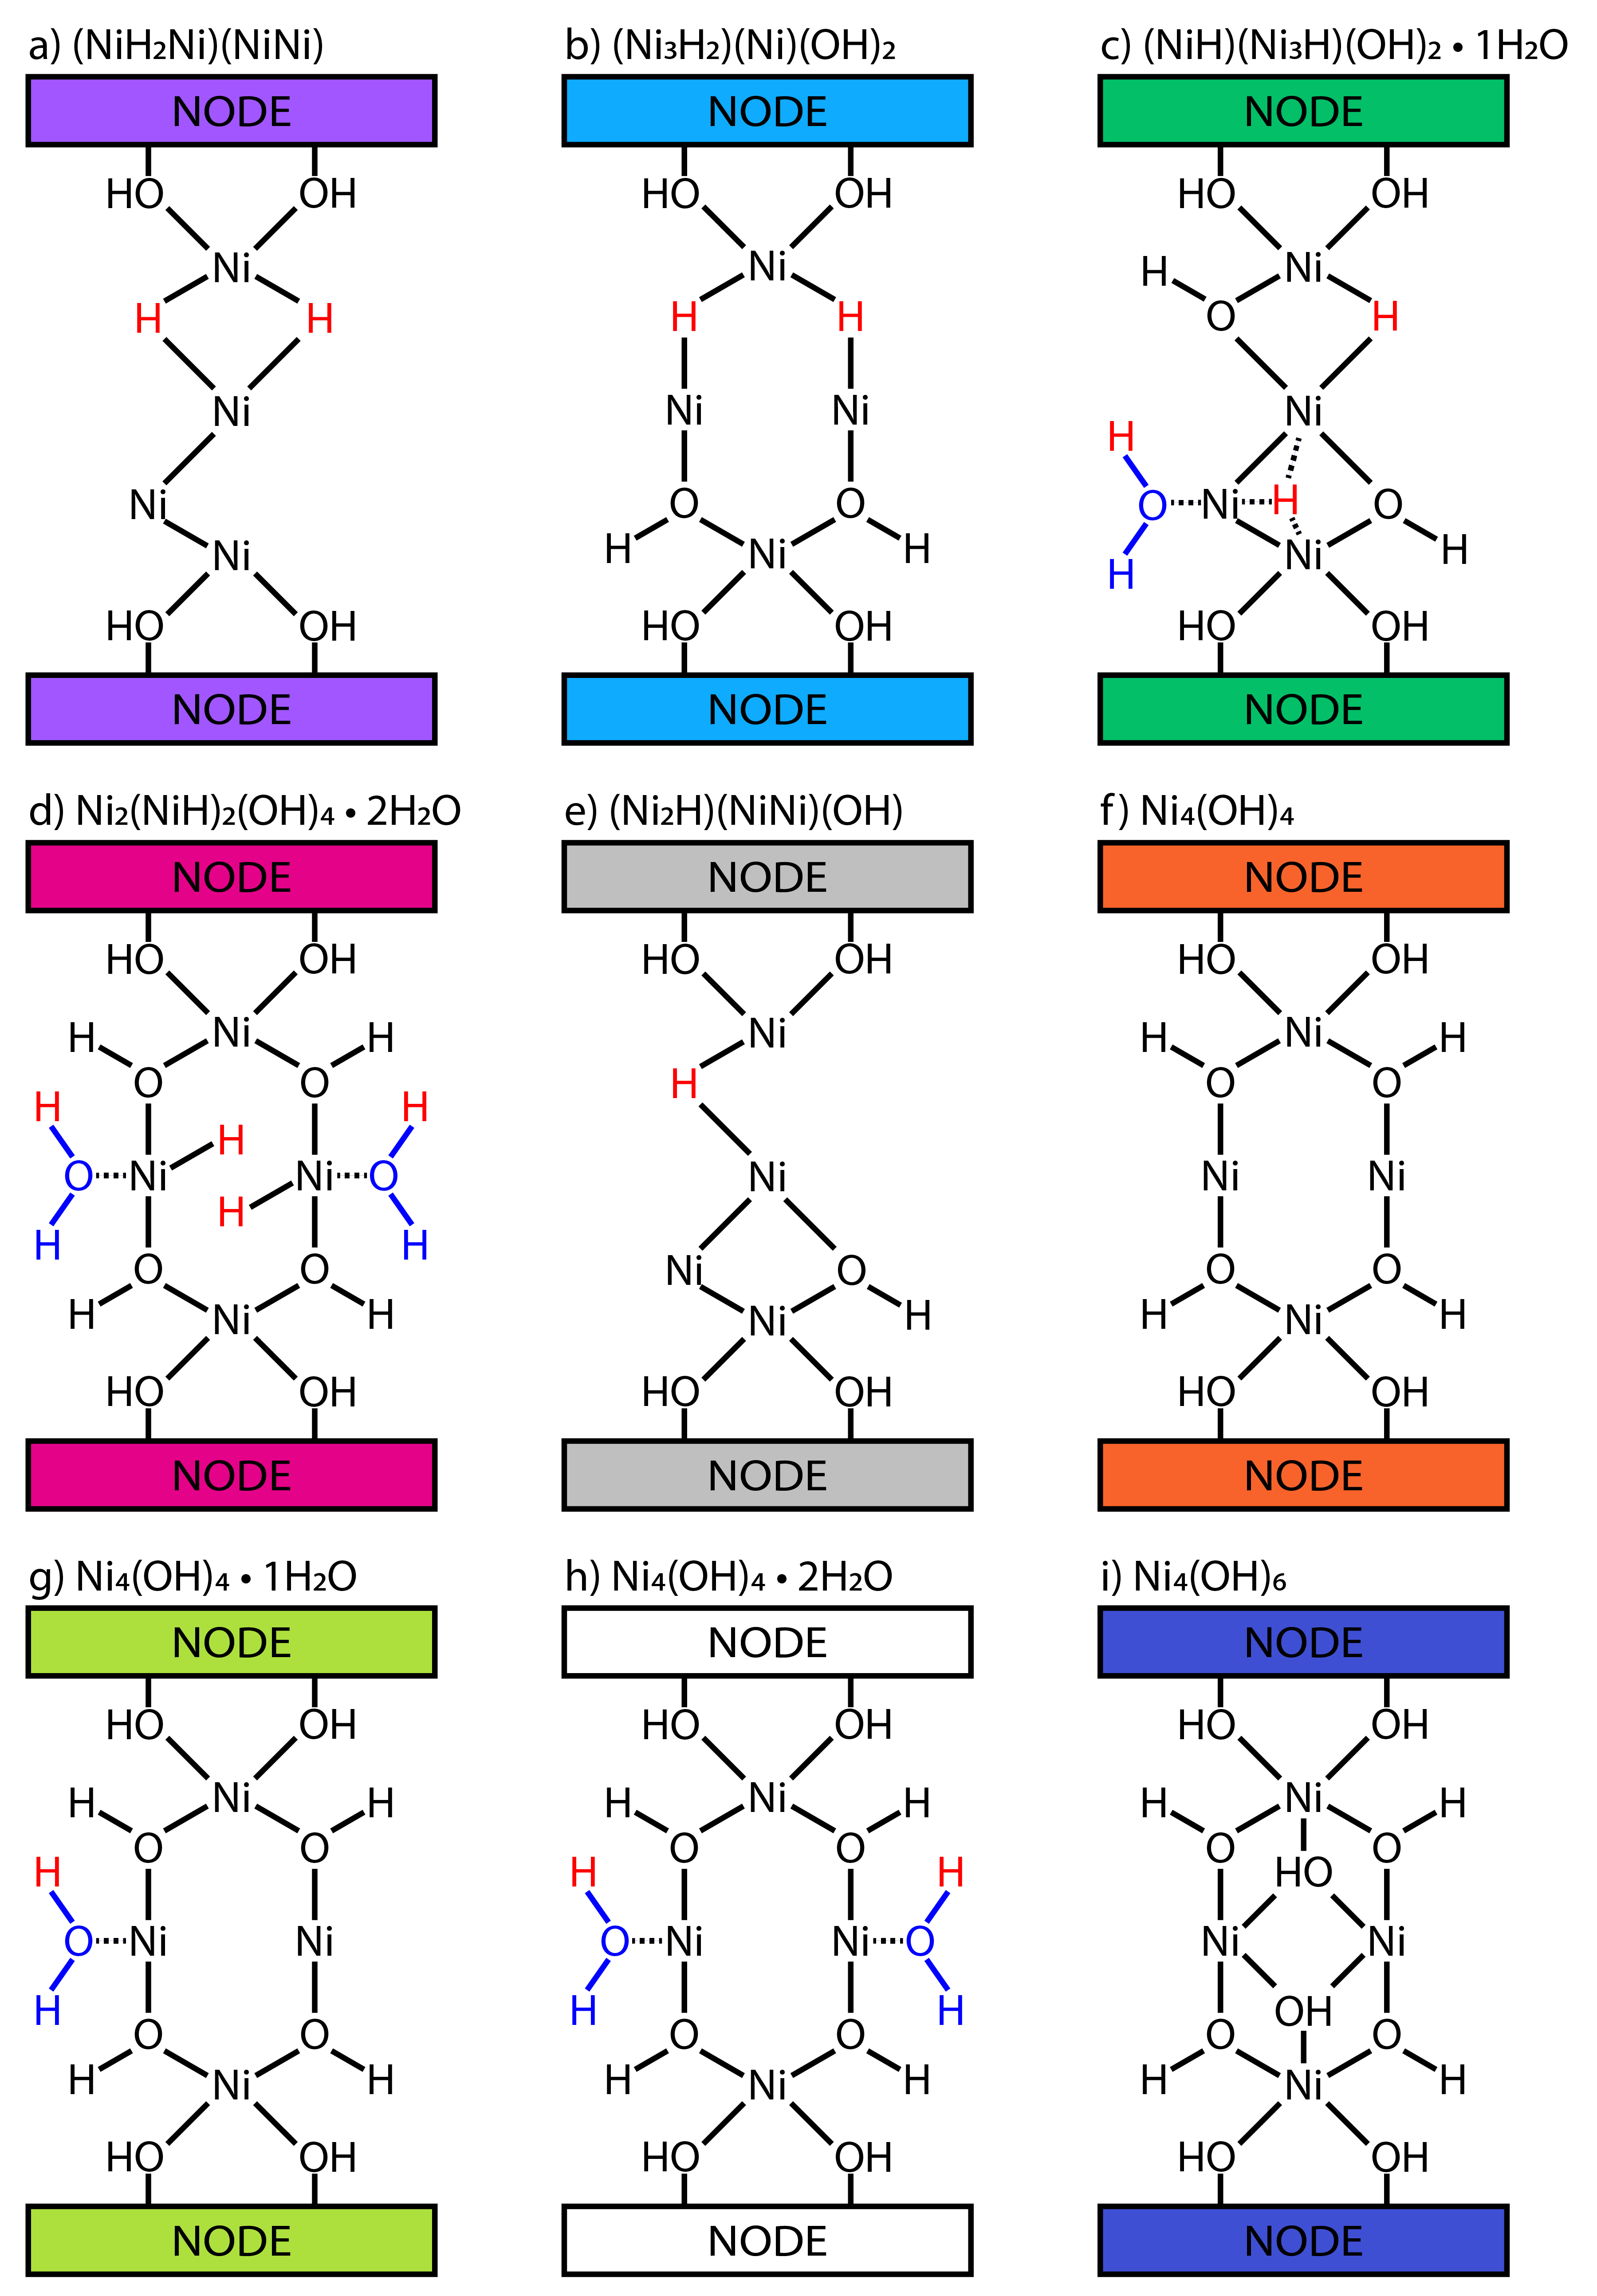
\includegraphics[width=0.80\textwidth]{zi-images/01-Ni-Graphics/2020-09-05-StructureDiagram-V05.png}
    \caption{Schematic representation of the lowest energy structures from the \textit{ab initio} thermodynamic analysis. The node colors scheme correspond to the \ce{Ni(II)} supported metal complex phase diagram.}
    \label{fig:structurediagramNi4}
\end{figure}

\newpage

\section{Discussion}
The structural characteristics of the supported metal complexes are dependent on the reaction conditions.
\begin{itemize}
    \item For the present results, we've determined the M(0) species based on the formation of the metallic bonds (bond distance) and the oxidation states matching the formal charge. Having an experimental Cu-Cu bond distance is good, because the computed bond distance is reasonable to between experimental (2.25 A) and theoretical (2.37 A). Those species are bound to the cluster still though (for both \ce{Cu} and \ce{Ni}). 
    \item Additional calculations being performed will remove the M(0) species as well as generate M-H on the single-site atoms in the cluster from partial stripping of the metal atoms. We will incorporate these structures into the analysis to address whether all metal atoms are being stripped from the node. Our current modeling results suggest that not all metal atoms are stripped from the node to form NPs. We are continuing to refine our model. 
    \item Are the M(0) species the mobile species suggested in Halder et al.? Presently, we refrain from calling them the mobile M(0) species. 
\end{itemize}

\newpage
\section{Future work}
A few comments from our previous email conversation a few weeks ago:
\begin{itemize}
    \item We are hoping to add your expertise at understanding the stability of both \ce{Cu3(OH)4} and \ce{Ni4(OH)6} cluster supported in NU-1000.
    \item For the Ni-Pt-NU-1000 project, the same \textit{ab initio} thermodynamic analysis approach could be applied to determine why \ce{CO} completely strips all \ce{Ni(II)} in Ni-NU-1000, but fails to remove \ce{Ni(II)} in Ni-Pt-NU-1000. Rather than a reservoir of \ce{H2} and \ce{H2O}, we could use a reservoir of \ce{CO}. The focus will be to determine why \ce{Pt} doping the node of NU-1000 suppresses the lose of \ce{Ni(II)} as \ce{Ni(CO)4}. With an understanding of why \ce{Pt} doping NU-1000 prevents \ce{Ni(II)} stripping, we might be able to propose alternative structural units to maintain \ce{Ni(II)} attachment without \ce{Pt}. 
    \item We could answer questions related to the catalytic activity of the \ce{CuIn} alloy NPs compared to the pure \ce{Cu} NPs. One of the Getman Group Postdocs is currently looking at the electrocatalytic reduction of \ce{CO} to \ce{CH3OH} on a \ce{Pt} surface under aqueous conditions. Using our modeling expertise, we could address why \ce{Cu} NPs can only reduce \ce{CO2} to \ce{CO}, but \ce{CuIN} NPs can reduce \ce{CO2} to \ce{CH3OH}. Our focus will be on understanding the synergistic effect of \ce{Cu} and \ce{In} in the \ce{CuIn} allow since neither one is capable of completely reducing \ce{CO2} to \ce{CH3OH}. 
\end{itemize}

\section{Additional questions}
We have the following list of primary questions:
\begin{itemize}
    \item When looking at the Cu-NU-1000 discussion, did you ever remove the Cu-NPs and determine whether the framework that was left behind was catalytically active? We wonder whether or not all the metal atoms are becoming the mobile \ce{M(0)} species. Are some metal atoms still attached to the node? 
    \item If you generate the \ce{Cu} single-site NU-1000 structures, do you still see the formation of \ce{Cu} NPs under reducing conditions?  
\end{itemize}  

\end{document}